\documentclass{article}
\usepackage{amsmath}
\usepackage{graphicx}

\begin{document}

\section{Scaling Laws}\label{sec:Scaling Laws}
The scaling laws used in this model are from \cite{housen2011ejecta}, which assume point-source crater evolution that applies to the final crater size, the growth of the transient crater and the majority of the observable ejecta field.

Depending on the size of the impact event, there are two separate cases: the strength regime and the gravity regime, discussed in Section \ref{ssec:Crater Size}. For smaller impacts, the strength regime dominates while for larger impacts, the gravity regime dominates. For materials that do not have a well defined strength (such as dry sand), the gravity regime dominates for all sizes of impacts.


%%%%%%%%%%%%%%%%%%%%%%%%%%%%%%%%%%%%%%%%%%%%%%%%%%%%%%%%%%%%%%%%%%%%%%
\subsection{Crater Size -- Strength \& Gravity Regime}\label{ssec:Crater Size}

The crater radius as determined by the \cite{housen2011ejecta} scaling laws is computed for both the strength and the gravity regime as the following:
\begin{equation}\label{eq:R gravity}
R\left(\frac{\rho}{m}\right)^{1/3} = H_2\left(\frac{\rho}{\delta}\right)^{\frac{1-3\nu}{3}}\left[\frac{Y}{\rho U^2}\right]^{-\frac{\mu}{2}},
\end{equation}
for the strength regime with $R$ the crater radius, $\rho$ the target bulk density, $m$ the impactor mass, $\delta$ the impactor bulk density, $Y$ the material strength (shear for granular targets and tensile for solid targets), and $U$ the normal component\footnote{See Section 5.2 of \cite{housen2011ejecta}.} of the impactor speed. See Table \ref{tab:scaling law parameters} for various scaling law parameters, and
\begin{equation}\label{eq:R strength}
R\left(\frac{\rho}{m}\right)^{1/3} = H_1\left(\frac{\rho}{\delta}\right)^{\frac{2+\mu-6\nu}{3(2+\mu)}}\left[\frac{ga}{U^2}\right]^{-\frac{\mu}{2+\mu}},
\end{equation}
for the gravity regime with $g = GM/r_m^2 = 1.625$ m s$^{-2}$ the lunar surface gravity, and $a$ the impactor radius.  

%%%%%%%%%%%%%%%%%%%%%%%%%%%%%%%%%%%%%%%%%%%%%%%%%%%%%%%%%%%%%%%%%%%%%%%
%\subsection{Minimum \& Maximum Ejected Speed}\label{ssec:Min Max Ejecta Speed}
%
%%%%%%%%%%%%%%%%%%%%%%%%%%%%%%%%%%%%%%%%%%%%%%%%%%%%%%%%%%%%%%%%%%%%%%%
%\subsection{Maximum Ejected Particle Mass}

%%%%%%%%%%%%%%%%%%%%%%%%%%%%%%%%%%%%%%%%%%%%%%%%%%%%%%%%%%%%%%%%%%%%%%
\subsection{Mass Ejected from Crater}\label{ssec:Mass Ejected from Crater}

The mass ejected from a crater by an impact can be summarized into two equations parameterized by the position from the crater center $x$ as
\begin{align}\label{eq:v/U}
\frac{v}{U} &= C_1\left[\frac{x}{a}\left(\frac{\rho}{\delta}\right)^\nu\right]^{-\frac{1}{\mu}}\left(1 - \frac{x}{n_2 R}\right)^p,\\
\frac{M}{m} &= \frac{3k}{4\pi}\frac{\rho}{\delta}\left[\left(\frac{x}{a}\right)^3-n_1^3\right],\label{eq:M_HH11}
\end{align}
for $n_1 a \le x \le n_2 R$, where $v$ is the ejecta speed (see Figures \ref{fig:v_vs_x_hidens} and \ref{fig:v_vs_x_lodens}), and $M$ is the mass ejected at speeds equal to or greater than $v$.



\begin{figure}[!htb]
	\centering
	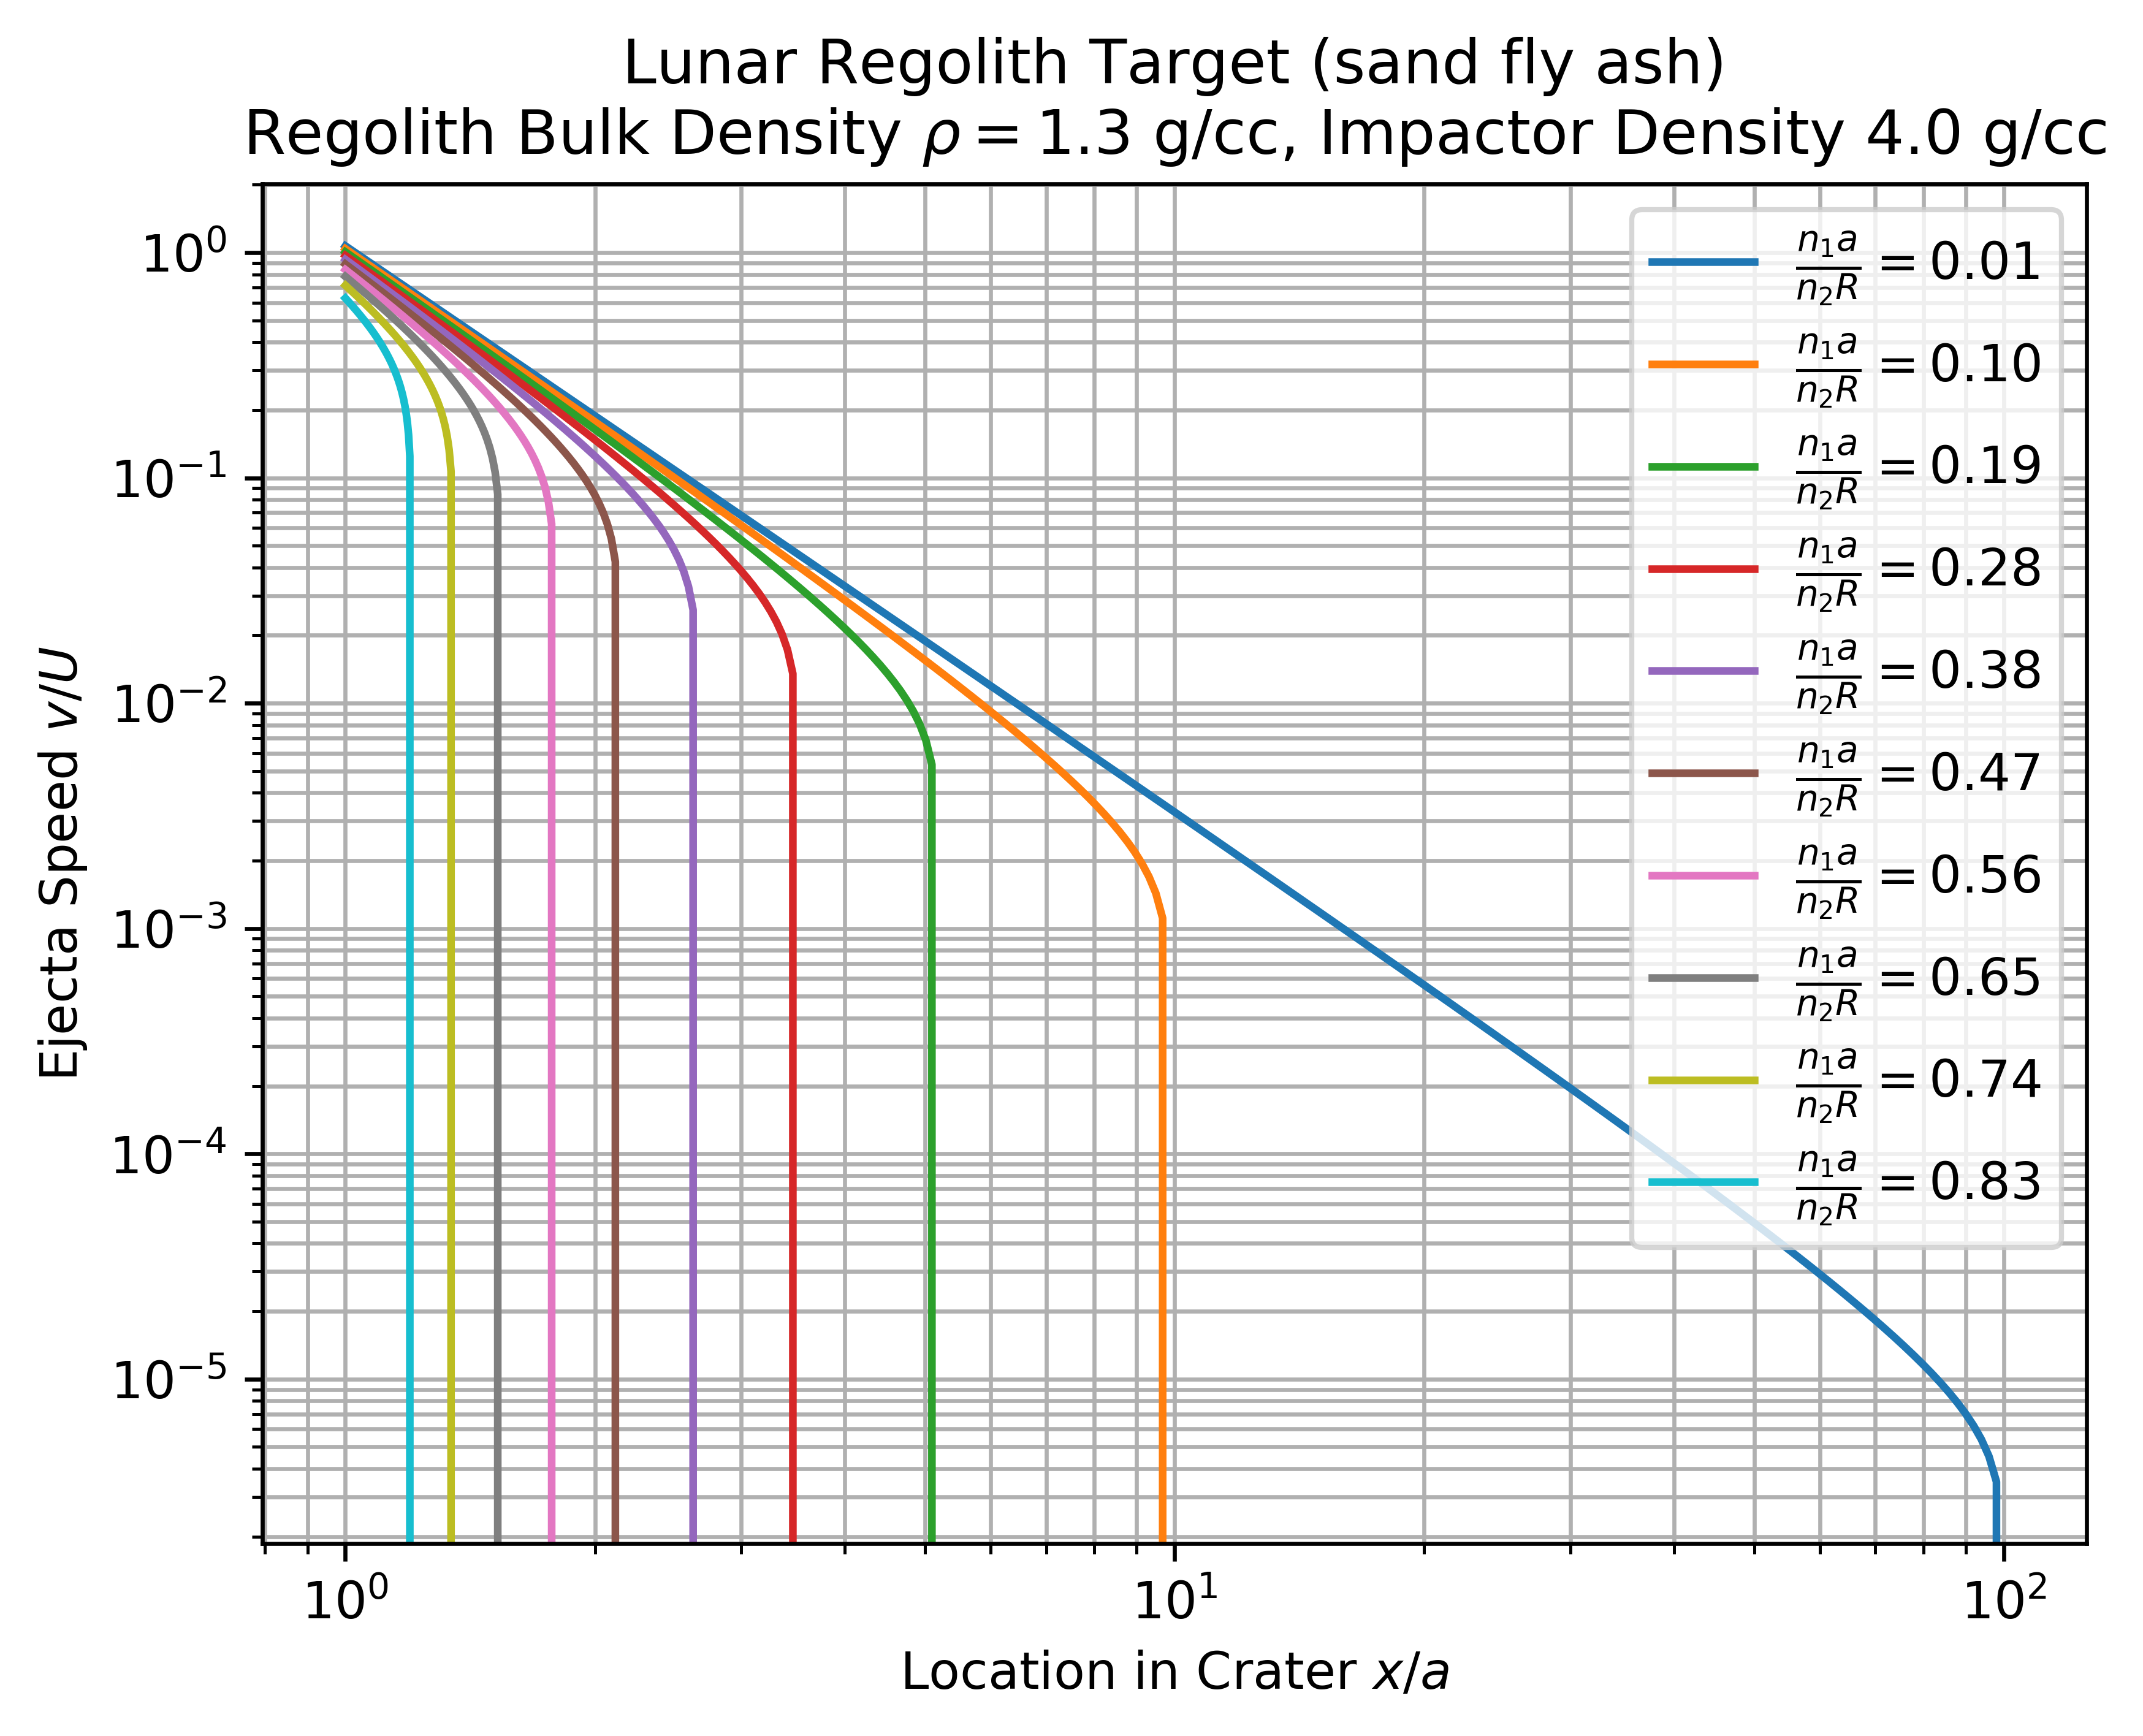
\includegraphics[width=0.65\linewidth]{v_vs_x_hidens.png}
	\caption{The ejecta speed $v/U$ (Equation \eqref{eq:v/U}) vs.\ location in the crater $x/a$ for a lunar regolith target (using SFA in Table~\ref{tab:scaling law parameters}) with regolith surface bulk density $\rho = 1.3$ g/cc and an impactor density of $4.0$ g/cc (e.g., MEM high density population). Each curve has a set effective impactor to crater radius $\frac{n_1 a}{n_2 R}$.}\label{fig:v_vs_x_hidens}
\end{figure}

\begin{figure}[!htb]
	\centering
	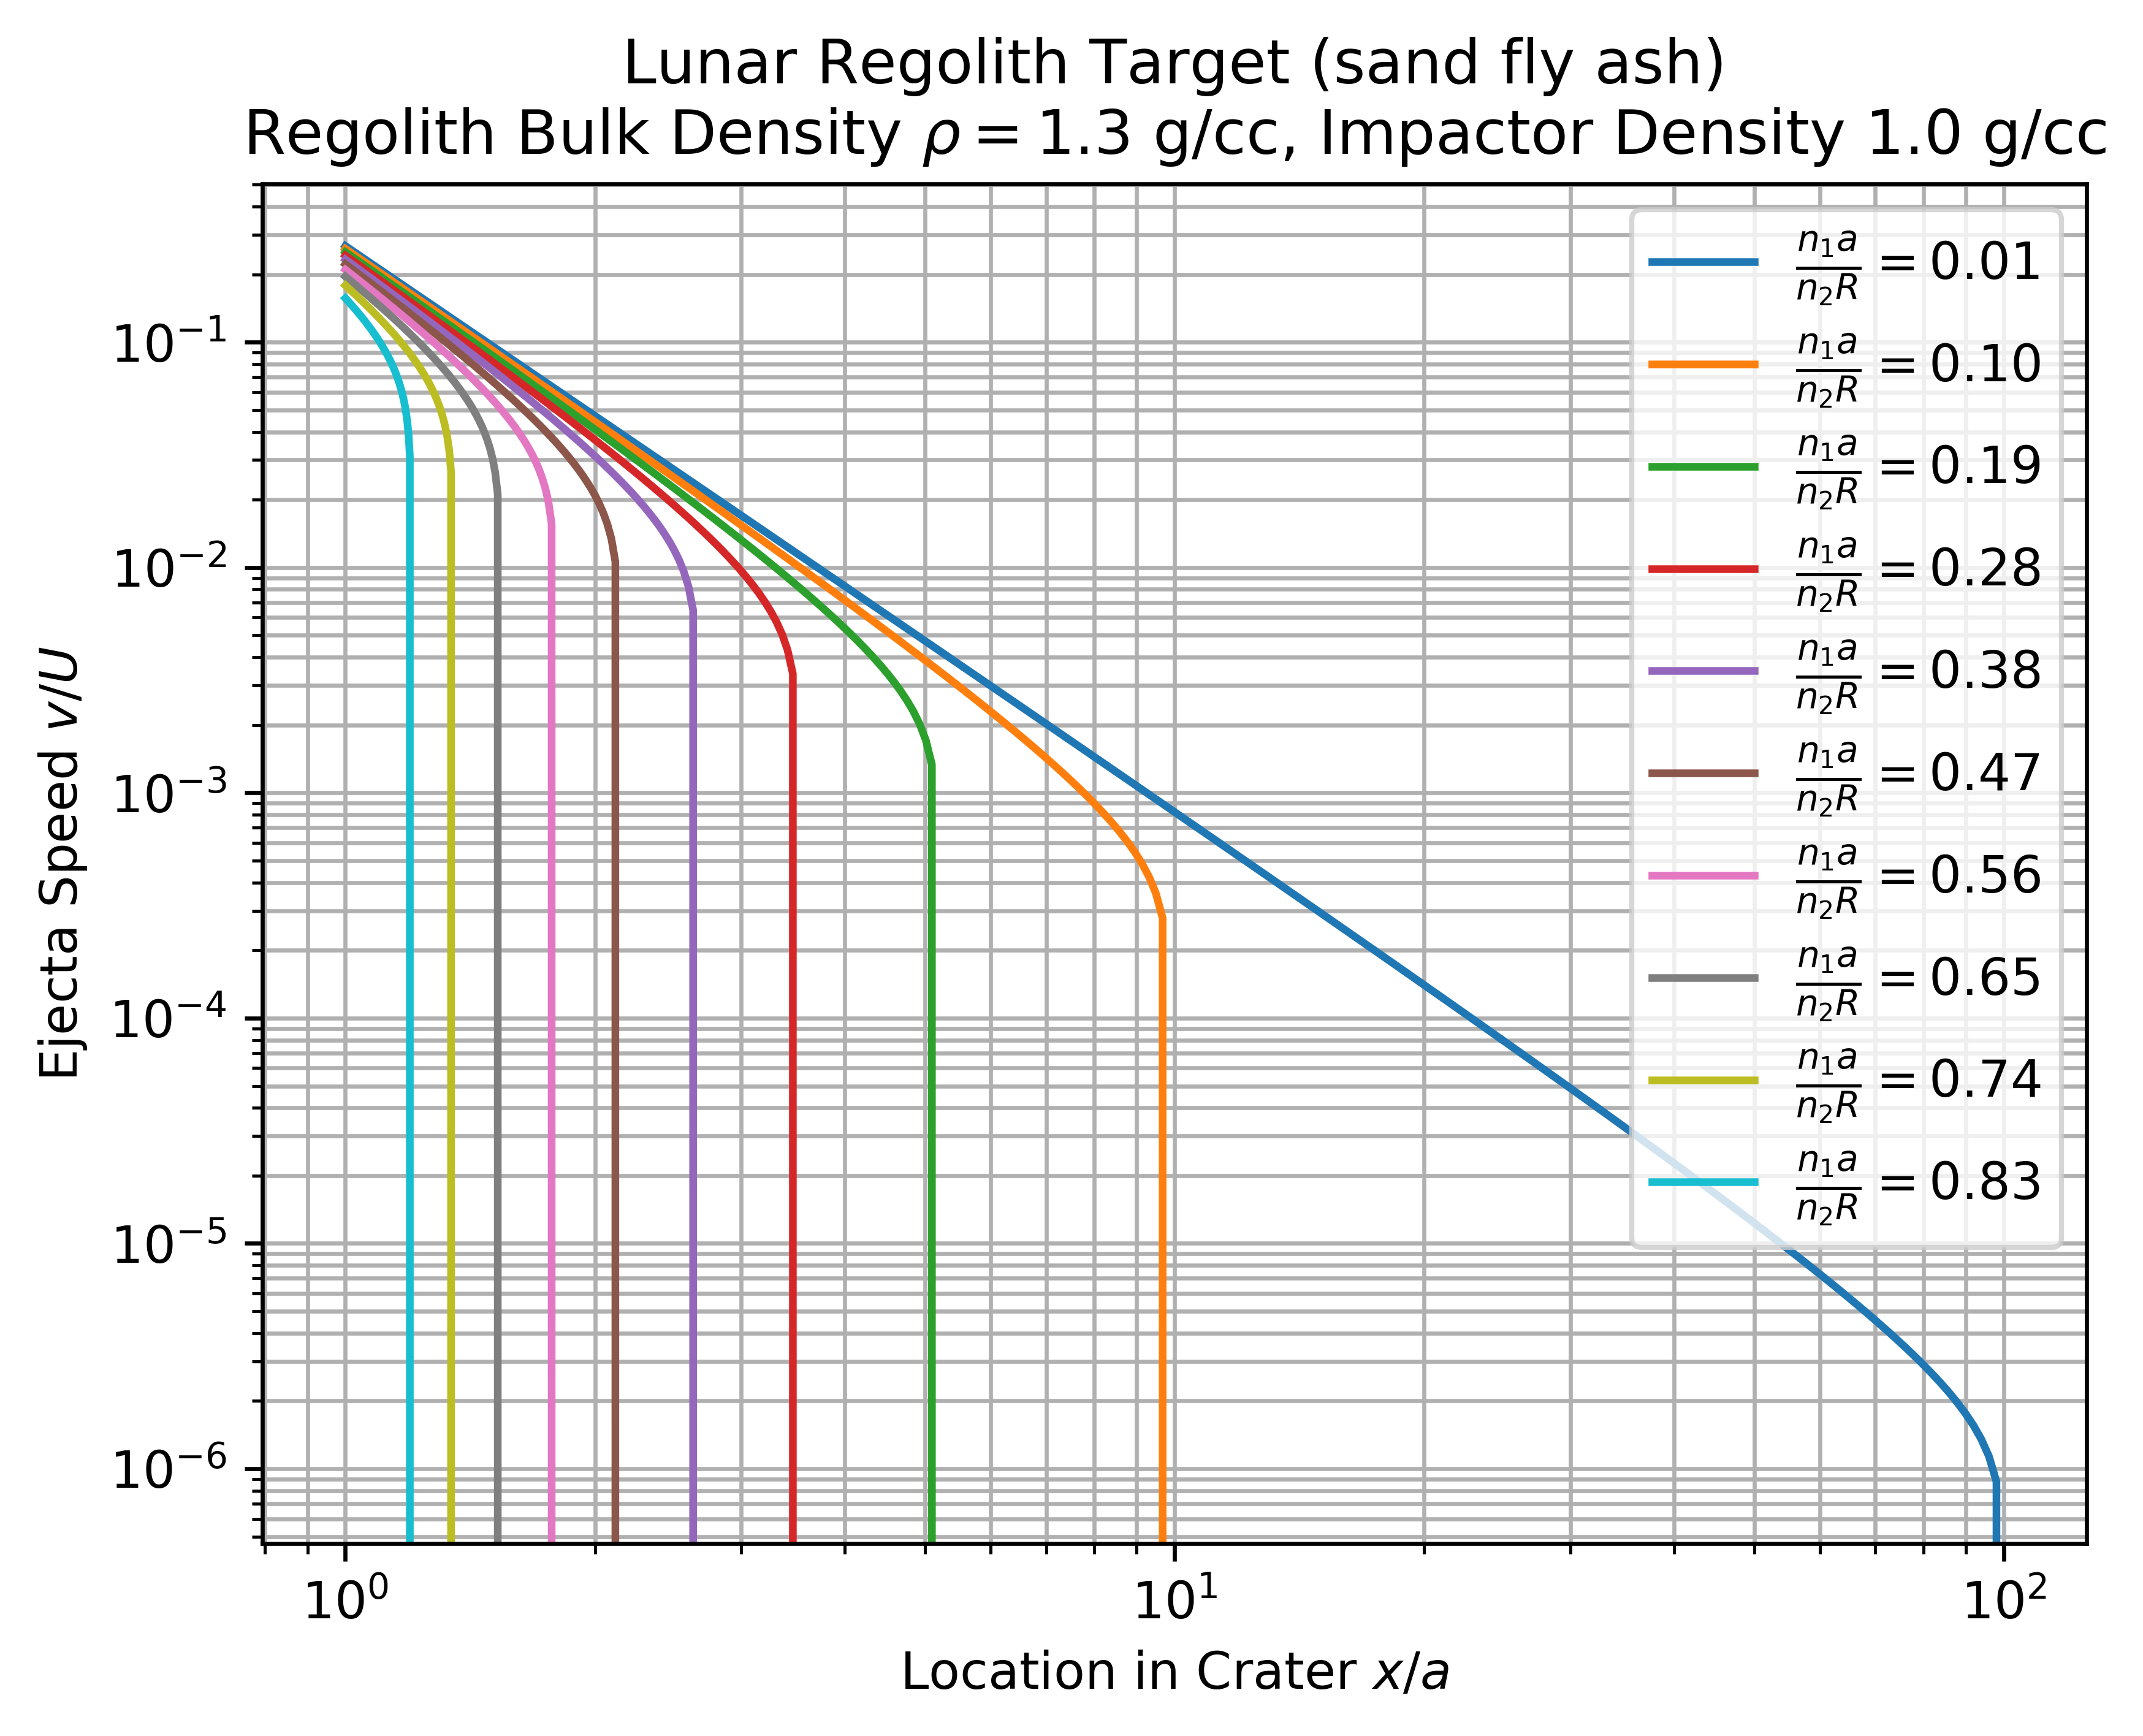
\includegraphics[width=0.65\linewidth]{v_vs_x_lodens.png}
	\caption{The ejecta speed $v/U$ (Equation \eqref{eq:v/U}) vs.\ location in the crater $x/a$ for a lunar regolith target (using SFA in Table~\ref{tab:scaling law parameters}) with regolith surface bulk density $\rho = 1.3$ g/cc and an impactor density of $1.0$ g/cc (e.g., MEM low density population). Each curve has a set effective impactor to crater radius $\frac{n_1 a}{n_2 R}$.}\label{fig:v_vs_x_lodens}
\end{figure}


The maximum speed occurs when $x = n_1 a$, or very close to ground zero, and is given by (see Figure \ref{fig:vmax_vs_x})
\begin{equation}\label{eq:vmax}
\frac{v_{max}}{U} = C_1\left[n_1\left(\frac{\rho}{\delta}\right)^\nu\right]^{-\frac{1}{\mu}}\left(1 - \frac{n_1 a}{n_2 R}\right)^p.
\end{equation}
If $v_{max} \le 0$, then it is assumed no ejecta was created by the impact.

\begin{figure}[!htb]
	\centering
	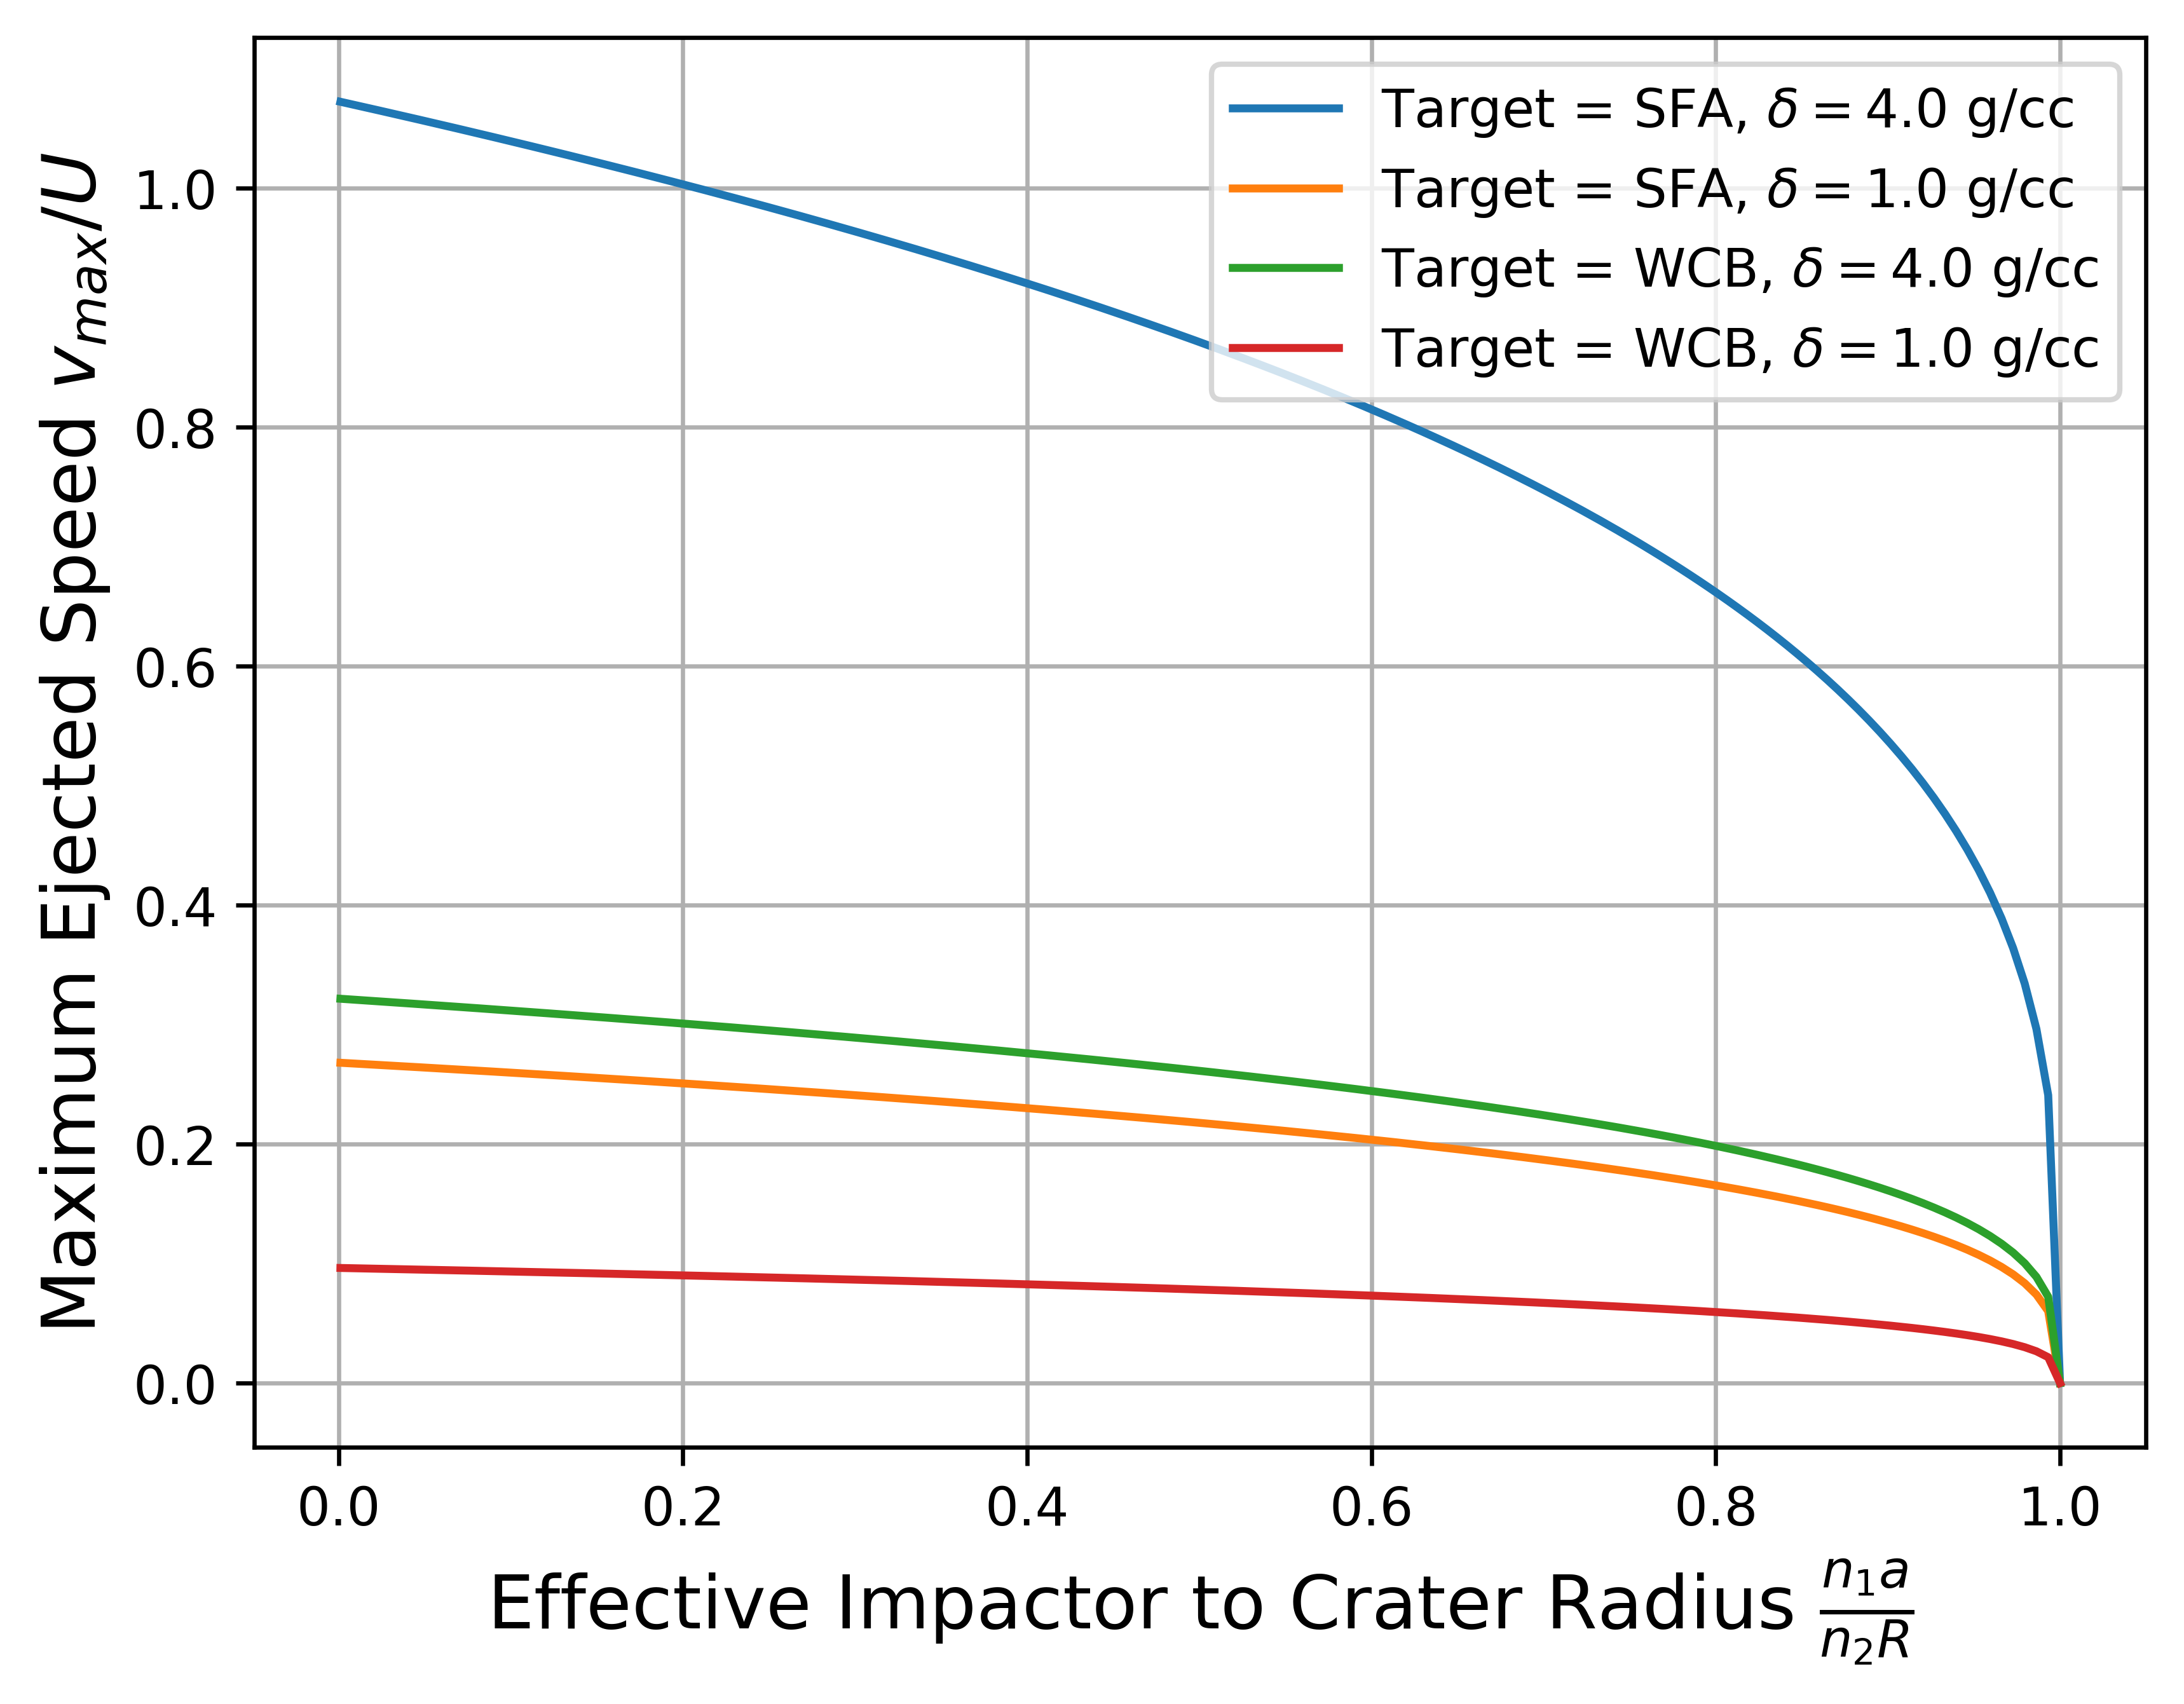
\includegraphics[width=0.65\linewidth]{vmax_vs_x.png}
	\caption{The ejecta speed $v/U$ (Equation \eqref{eq:v/U}) vs.\ effective impactor to crater radius $\frac{n_1 a}{n_2 R}$ for a lunar regolith target (using SFA and WCB in Table~\ref{tab:scaling law parameters}) with regolith surface bulk density $\rho = 1.3$ g/cc and an impactor density of $1.0$ and $4.0$ g/cc (e.g., MEM low and high density populations).}\label{fig:vmax_vs_x}
\end{figure}




The total mass ejected is given when $x = n_2 R$,
\begin{equation}\label{eq:Mtot}
\frac{M_{tot}}{m} = \frac{3k}{4\pi}\frac{\rho}{\delta}\left[\left(\frac{n_2 R}{a}\right)^3-n_1^3\right].
\end{equation}
It is equivalent to say that if $M_{tot} \le 0$, then no ejecta was created by the impact.

The ejecta speed $v$ and mass of ejecta at speeds $v$ or greater $M$, can also be written in terms of the maximum speed $v_{max}$ and total ejected mass $M_{tot}$ as
\begin{equation}\label{eq:v/v_max}
\frac{v}{v_{max}} = \left(\frac{x}{n_1 a}\right)^{-\frac{1}{\mu}}\frac{\left(1-\frac{x}{n_2 R}\right)^p}{\left(1-\frac{n_1 a}{n_2 R}\right)^p},
\end{equation}
and
\begin{equation}\label{M/M_tot}
\frac{M}{M_{tot}} = \frac{\left(\frac{x}{n_2 R}\right)^3 - \left(\frac{n_1 a}{n_2 R}\right)^3}{1 - \left(\frac{n_1 a}{n_2 R}\right)^3}.
\end{equation}
%\clearpage
\subsubsection{Ejected Mass Distribution}

The differential mass, or ejecta mass distribution, in terms of the speed can be computed using the chain rule as follows:
\begin{equation}\label{eq:dM/dv chain rule}
\frac{dM}{dv} = \frac{dM}{dx}\frac{dx}{dv} = \frac{dM}{dx}\left(\frac{dv}{dx}\right)^{-1}.
\end{equation}
The first term can be calculated from Equation \eqref{eq:M_HH11} such that
\begin{equation}\label{eq:dM/dx}
\frac{dM}{dx} = \frac{9k}{4\pi}\frac{\rho}{\delta}\left(\frac{x}{a}\right)^2\frac{m}{a},
\end{equation}
and the second term from Equation \eqref{eq:v/U}, giving
\begin{equation}\label{eq:dv/dx}
\frac{dv}{dx} = -C_1\left[\frac{x}{a}\left(\frac{\rho}{\delta}\right)^\nu\right]^{-\frac{1}{\mu}}\left(1 - \frac{x}{n_2 R}\right)^p
\frac{1+(\mu p -1)\frac{x}{n_2 R}}{\mu\left(1-\frac{x}{n_2 R}\right)}\frac{U}{x}.
\end{equation}
Therefore, the differential mass is found by taking Equation \eqref{eq:dM/dx} divided by Equation~\eqref{eq:dv/dx} giving
\begin{equation}\label{eq:dM/dv final}
\frac{dM}{dv} = -\frac{9k}{4\pi}\frac{\rho}{\delta}\left(\frac{x}{a}\right)^3\frac{\mu\left(1-\frac{x}{n_2 R}\right)}{1+(\mu p-1)\frac{x}{n_2 R}}\frac{m}{v}.
\end{equation}



%%%%%%%%%%%%%%%%%%%%%%%%%%%%%%%%%%%%%%%%%%%%%%%%%%%%%%%%%%%%%%%%%%%%%%
\subsection{Scaling Law Parameters}\label{ssec:Scaling Law Parameters}
%In the meteoroid ejecta model described in this document, the scaling laws from \cite{housen2011ejecta} are employed. In this section, the parameters of various material types used in fits to the scaling laws are summarized. The specific scaling law equations are discussed in Section \ref{sec:Scaling Laws}.

The various sets of parameters for different target materials are given in Table 3 of \cite{housen2011ejecta} with most of them copied here in Table \ref{tab:scaling law parameters}, with undefined values filled in that are best represented by either solid, semi-solid, or fine material where applicable. If a material has zero strength, the crater scaling is automatically in the gravity regime and there is no strength regime (and no need for $H_2$ to be defined).


\begin{table}[!htb]
	\begin{center}
		\caption{Summary of constants used in the \cite{housen2011ejecta} ejecta model.}
		\label{tab:scaling law parameters}
		\begin{tabular}{l l l l l l l l l}
			\hline
			Curve no.\ & C1    & C2   & C3  & C4   & C5   & C6  & C7  & C8  \\
			\hline
			Target     & Water & Rock & WCB & Sand & Sand & GMS & SFA & PS\\
			Porosity   & $\sim 0$ & $\sim 0$ & $20\%$ & $35\pm 5\%$ & $35\pm 5\%$ & $36\%$ & $45\%$ & $60\%$\\
			$\mu$ & $0.55$ & $0.55$ & $0.46$ & $0.41$ & $0.41$ & $0.45$ & $0.4$ & $0.35$\\
			$C_1$ & $1.5$ & $1.5$ & $0.18$ & $0.55$ & $0.55$ & $1.0$ & $0.55$ & $0.6$ \\
			$k$ & $0.2$ & $0.3$ & $0.3$ & $0.3$ & $0.3$ & $0.5$ & $0.3$ & $0.32$\\ 
			$H_1$ & $0.68$ & $0.68^{*1}$ & $0.5^{*2}$ & $0.59$ & $0.59$ & $0.8$ & $0.59^{*3}$ & $0.59^{*3}$\\
			$H_2$ & -- & $1.2$ & $0.38$ & -- & -- & -- & $0.4$ & $0.81$\\
			$n_{2,G}$ & $1.5$ & $1.5$ & $1.3^{*3}$ & $1.3$ & $1.3$ & $1.3$ & $1.2^{*2}$ & $1.2^{*2}$\\
			$p$ & $0.5$ & $0.5$ & $0.3$ & $0.3$ & $0.3$ & $0.3$ & $0.3$ & $0.2$\\
			$Y$ (MPa) & $0$ & $30$ & $0.45$ & $0$ & $0$ & $0$ & $4\times 10^{-3}$ & $2\times 10^{-3}$\\
			\hline
			\multicolumn{9}{l}{\footnotesize Note: WCB = weakly cemented basalt, GMS = glass micro-spheres, PS = perlite/sand mixture,} \\
			\multicolumn{9}{l}{\footnotesize SFA = sand/fly ash. All cases shown in this table used: $\nu=0.4$, $n_1=1.2$, $n_{2,S} = 1$, $g=9.81$ m/s$^2$.} \\
			\multicolumn{9}{l}{\footnotesize $*1$ from water, $*2$ no value given, $*3$ from sand.}\\
			
		\end{tabular}
	\end{center}
\end{table}

The average regolith porosity from $0$ -- $60$ cm is $46\pm 2 \%$ (see Table \ref{tab:porosity}), so the set of parameters that define SFA (sand/fly ash) are adopted. For a higher fidelity strength, Equation \eqref{eq:shear strength_avg_para} can be used instead of $Y = 4$ kPa.





\end{document}